\documentclass[12pt]{article}
\usepackage[a4paper,margin=1in,footskip=0.25in]{geometry} % set margins
\usepackage[portuguese]{babel}
\usepackage[utf8]{inputenc}
\usepackage{hyperref} 
\usepackage{amsmath}
\usepackage{amssymb}
\usepackage{amsthm}
\usepackage{graphicx}    % needed for include graphics
\usepackage{subfigure}   % add subfigures
\usepackage{indentfirst}
\usepackage{float}       % needed for [H] figure placement option
\usepackage{setspace}    % needed for doublespacing
\usepackage{tikz}
\usepackage{algpseudocode}

% Macros
\renewcommand{\familydefault}{\sfdefault} % sans-serif
\newcommand{\lowtext}[1]{$_{\text{#1}}$}

% Adds ./img/ to the path of figures
\graphicspath{{./img/}}

\title{Relatório EP1 - MAC0219}
\author{Bruno Sesso, Gustavo Estrela de Matos, Lucas Sung Jun Hong}

\begin{document}
% Espaçamento duplo 
\doublespacing
\begin{titlepage}
    \vfill
    \begin{center}
        \vspace{0.5\textheight}
        \noindent
        Instituto de Matemática e Estatística \\
        EP1 - MAC0219 \\
        \vfill
        \noindent
        {\Large Cálculo do Conjunto de Mandelbrot
        em Paralelo com Pthreads e OpenMP} \\
        \bigskip
        \bigskip
        \begin{tabular}{ll}
            {\bf Professor:} & {Alfredo Goldman} \\
            {\bf Alunos:}    & {Bruno Sesso} \\
                             & {Gustavo Estrela de Matos} \\
                             & {Lucas Sung Jun Hong} \\
        \end{tabular} \\
        \vspace{\fill}
       \bigskip
        São Paulo, \today \\
       \bigskip
    \end{center}
\end{titlepage}

\pagebreak
\tableofcontents
\pagebreak

\section{Introdução}
\section{Código Sequencial}
\section{Código em OpenMP}


\section{Código em Pthreads}
Utilizamos duas diferentes abordagens para paralelizar o código com
o uso de pthreads, tentando se aproximar ao comportamento do OpenMP e 
suas diretivas {\em omp parallel for schedule (dynamic)} e {\em omp 
parallel for schedule (static)}. As diferenças de funcionamento dos 
dois códigos está na maneira em que o trabalho é dividido e como ele é
distribuido para cada thread.

\subsection{Implementação com Divisão Estática}
Chamamos de implementação com divisão estática a versão do nosso 
código em pthreads no qual o trabalho é dividido em $n$ pedaços de mesmo 
tamanho, e cada pedaço é dado a uma thread. Chamamos essa implementação
de estática porque cada thread recebe apenas um bloco de trabalho,
pré-determinado pela divisão feita, que será processado do começo ao
fim (no escopo da thread) pela mesma thread.

Para implementar esse código, precisamos apenas construir uma estrutura
de dados que era capaz de guardar um bloco de pixels a ser calculado.
Dado essa estrutura, basta criar uma thread para cada bloco de trabalho,
que por sua vez deve calcular os pixels correspondentes e atualizar o 
buffer de cores.

Devemos observar que essa implementação pode implicar em threads ociosas
enquanto outras estão trabalhando. Como a quantidade de iterações
necessárias para se calcular o valor de um pixel varia, é possível que
um bloco de pixels seja calculado muito mais rápido do que outro; 
imagine por exemplo um bloco onde cada ponto calculado diverge 
rápidamente e outro bloco onde isso não acontece. Portanto, como a 
divisão de trabalho é estática, é provável que uma thread termine seu
trabalho muito antes de outra, o que significa em um uso não muito bom
de recursos da máquina.

Uma possível solução para esse problema seria o aumento no número de 
threads, o que cria uma fragmentação maior do trabalho. Essa 
fragmentação ameniza o problema anterior porque divide mais o trabalho,
deixando menor a diferença de tempo necessário para se calcular cada 
parte. Entretanto, criar um número excessivo de threads pode dar mais
trabalho ao escalonador do sistema operacional, que deve lidar com 
várias linhas de processamento.

\begin{figure}[!ht]
    \centering
    \begin{tabular}{c c}
        \subfigure[] {\scalebox{.35}{
            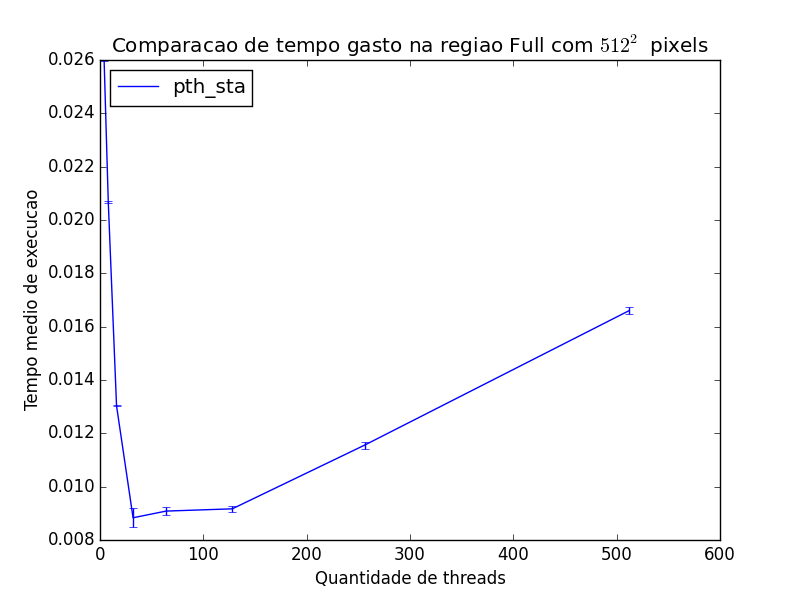
\includegraphics{time_x_thread_numpth_sta_n512.png}}
            \label {fig:higher_thread_num:A}
        }
        &
        \subfigure[] {\scalebox{.35}{
            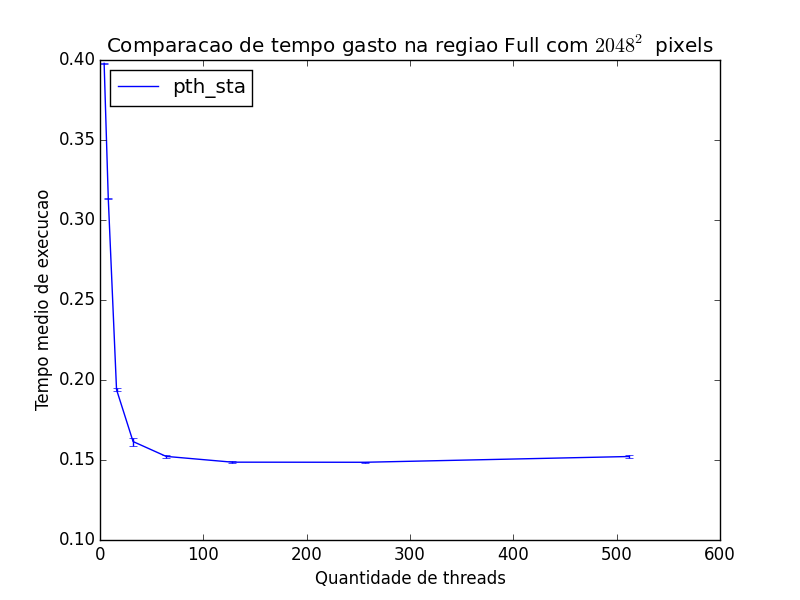
\includegraphics{time_x_thread_numpth_sta_n2048.png}}
            \label {fig:higher_thread_num:B}
        }

    \end{tabular}
    \caption{É possível notar em ambas figuras que o aumento do número
    de threads de fato diminui o tempo de execução do programa. No 
    gráfico \ref{fig:higher_thread_num:A} fica evidente que o tempo 
    gasto no controle das threads pode afetar o tempo de execução do
    programa.}
    \label{fig:higher_thread_num} 
\end{figure}



\subsection{Implementação com Divisão Dinâmica}

\section{Discussões Gerais}
\section{Conclusão}
\end{document}
